\documentclass[a4paper, 12pt]{article}%тип документа

%%%Библиотеки
	%\usepackage[warn]{mathtext}	
	\usepackage[T2A]{fontenc} % кодировка
	\usepackage[utf8]{inputenc} % кодировка исходного текста
	\usepackage[english,russian]{babel} % локализация и переносы
	\usepackage{caption}
	\usepackage{listings}
	\usepackage{amsmath,amsfonts,amssymb,amsthm,mathtools}
	\usepackage{wasysym}
	\usepackage{graphicx}%Вставка картинок правильная
	\usepackage{float}%"Плавающие" картинки
	\usepackage{wrapfig}%Обтекание фигур (таблиц, картинок и прочего)
	\usepackage{fancyhdr} %загрузим пакет
	\usepackage{lscape}
	\usepackage{xcolor}
	\usepackage[normalem]{ulem}
	\usepackage{hyperref}

%%%Конец библиотек




%%%Настройка ссылок
	\hypersetup
	{
		colorlinks=true,
		linkcolor=blue,
		filecolor=magenta,
		urlcolor=blue
	}
%%%Конец настройки ссылок


%%%Настройка колонтитулы
	\pagestyle{fancy}
	\fancyhead{}
	\fancyhead[L]{Лабораторная работа}
	\fancyhead[R]{Талашкевич Даниил, группа Б01-009}
	\fancyfoot[C]{\thepage}
%%%конец настройки колонтитулы



							\begin{document}
						%%%%Начало документа%%%%


%%%Начало титульника
\begin{titlepage}

	\newpage
	\begin{center}
		\normalsize Московский физико-технический институт \\(госудраственный 			университет)
	\end{center}

	\vspace{6em}

	\begin{center}
		\Large Лабораторная работа по электричеству\\
	\end{center}

	\vspace{1em}

	\begin{center}
		\large \textbf{Релаксационные колебания [3.2.8]}
	\end{center}

	\vspace{2em}

	\begin{center}
		\large Талашкевич Даниил Александрович\\
		Группа Б01-009
	\end{center}

	\vspace{\fill}

	\begin{center}
	Долгопрудный \\2021
	\end{center}
	
\end{titlepage}
%%%Конец Титульника



%%%Настройка оглавления и нумерации страниц
	\thispagestyle{empty}
	\newpage
	\tableofcontents
	\newpage
	\setcounter{page}{1}
%%%Настройка оглавления и нумерации страниц


					%%%%%%Начало работы с текстом%%%%%%

\section{Аннотация}
 
$\quad\ \ \textbf{Цель работы}$: изучение вольт-амперной характеристики нормального тлеющего разряда; исследование релаксационного генератора на стабилитроне.

$\textbf{В работе используются}$: стабилитрон СГ-2 (газонаполненный диод) на монтажной панели, магазин ёмкостей, магазин сопротивлений, источник питания, амперметр, вольтметр, осциллограф.

В работе предлагается снять вольт-амперную характеристику стабилитрона и познакомиться с работой релаксационного генератора: определить критическое сопротивление, исследовать зависимость периода колебаний от сопротивления при фиксированной ёмкости и от ёмкости при фиксированном сопротивлении.

\section{Теоретические сведения}

 Колебательные системы, как правило, имеют два накопителя, между которыми происходит перекачка энергии. В контуре, содержащем конденсатор и катушку индуктивности, электрическая энергия переходит в магнитную и обратно; при колебаниях маятника потенциальная энергия поля тяжести переходит в кинетическую энергию движущейся массы и т.д. 

\begin{wrapfigure}{r}{0.3\textwidth} 
\begin{center}
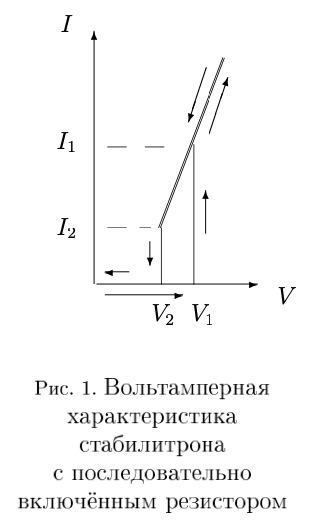
\includegraphics[width=0.3\textwidth]{./ann/1.PNG} 
\end{center}
\end{wrapfigure}

Встречаются, однако, колебательные системы, содержащие всего один накопитель энергии. Рассмотрим в качестве примера электрическую цепь, содержащую конденсатор и сопротивление без самоиндукции. Разряд конденсатора через сопротивление представляет собой апериодический процесс. Разряду, однако, можно придать периодический характер, возобновляя заряд конденсатора через постоянные промежутки времени. Колебания в этом случае являются совокупностью двух апериодических процессов - процесса зарядки конденсатора и процесса его разрядки. Такие колебания называются релаксационними.\\
В нашей установке роль ключа, обеспечивающего последовательно попеременную зарядку и разрядку конденсатора, играет газоразрядный диод. Зависимость тока от напряжения для газоразрядной лампы не подчиняется закону Ома и характеризуется рядом особенностей (рис. 1). При малых напряжениях лампа не пропускает тока вовсе (не горит). Ток в лампе возникает только в том случае, если разность потенциалов на её электродах достигает напряжения зажигания $V_{1} .$ При этом, тлеюиций разряд. При дальнейшем незначительном увеличении напряжения сила тока заметно возрастает по закону, близкому к линейному. 
Если начать уменьшать напряжение на горящей лампе, то при напряжении, равном $V_{1},$ лампа ещё не гаснет, и сила тока продолжает уменьшаться. Лампа перестанет пропускать ток лишь при напряжении гашения $V_{2},$ которое обычно существенно меньше $V_{1}$. Сила тока при этом скачком падает от значения $I_{2}\left(I_{2}<I_{1}\right)$ до нуля. Характеристика, изображённая на рис. 1, несколько идеализирована. $\mathrm{Y}$ реальной лампы зависимость $I(V)$ не вполне линейна. При $V>V_{1}$ графики
соответствующие возрастанию и убыванию напряжения, не всегда совпадают. Эти отличия, впрочем, носят второстепенный характер и для нашей задачи несущественны.
 
\newpage

\begin{wrapfigure}{r}{0.3\textwidth} 
\begin{center}
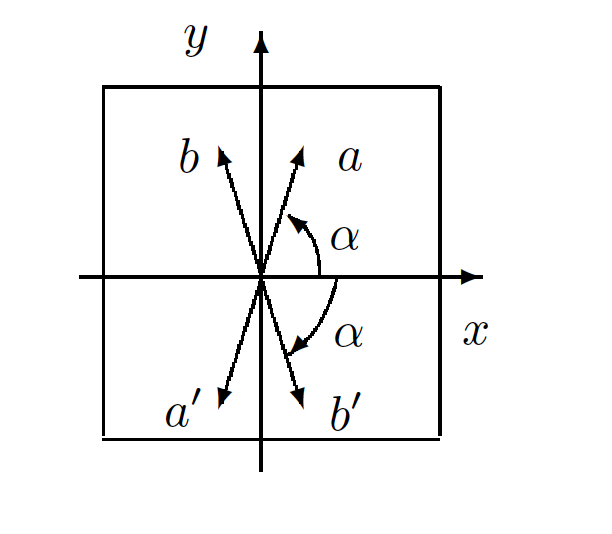
\includegraphics[width=0.3\textwidth]{./ann/2.PNG} 
\end{center}
\end{wrapfigure}


Рассмотрим схему релаксационного генератора, представленную на рис. $2 .$ Пусть напряжение бата- реи $U$ больше напряжения зажигания $V_{1} .$ В обозначениях, принятых на схеме, справедливо уравнение

$$I_{C}+I(V)=\frac{U-V}{R}$$

$$C \frac{d V}{d T}+I(V)=\frac{U-V}{R}$$
\\

В стационарном режиме работы, когда напряжение $V$ на конденсаторе постоянно и $d V / d t=0,$ ток через лампу равен

$$I_{\mathrm{cr}}=\frac{U-V}{R}$$

\begin{wrapfigure}{r}{0.3\textwidth} 
\begin{center}
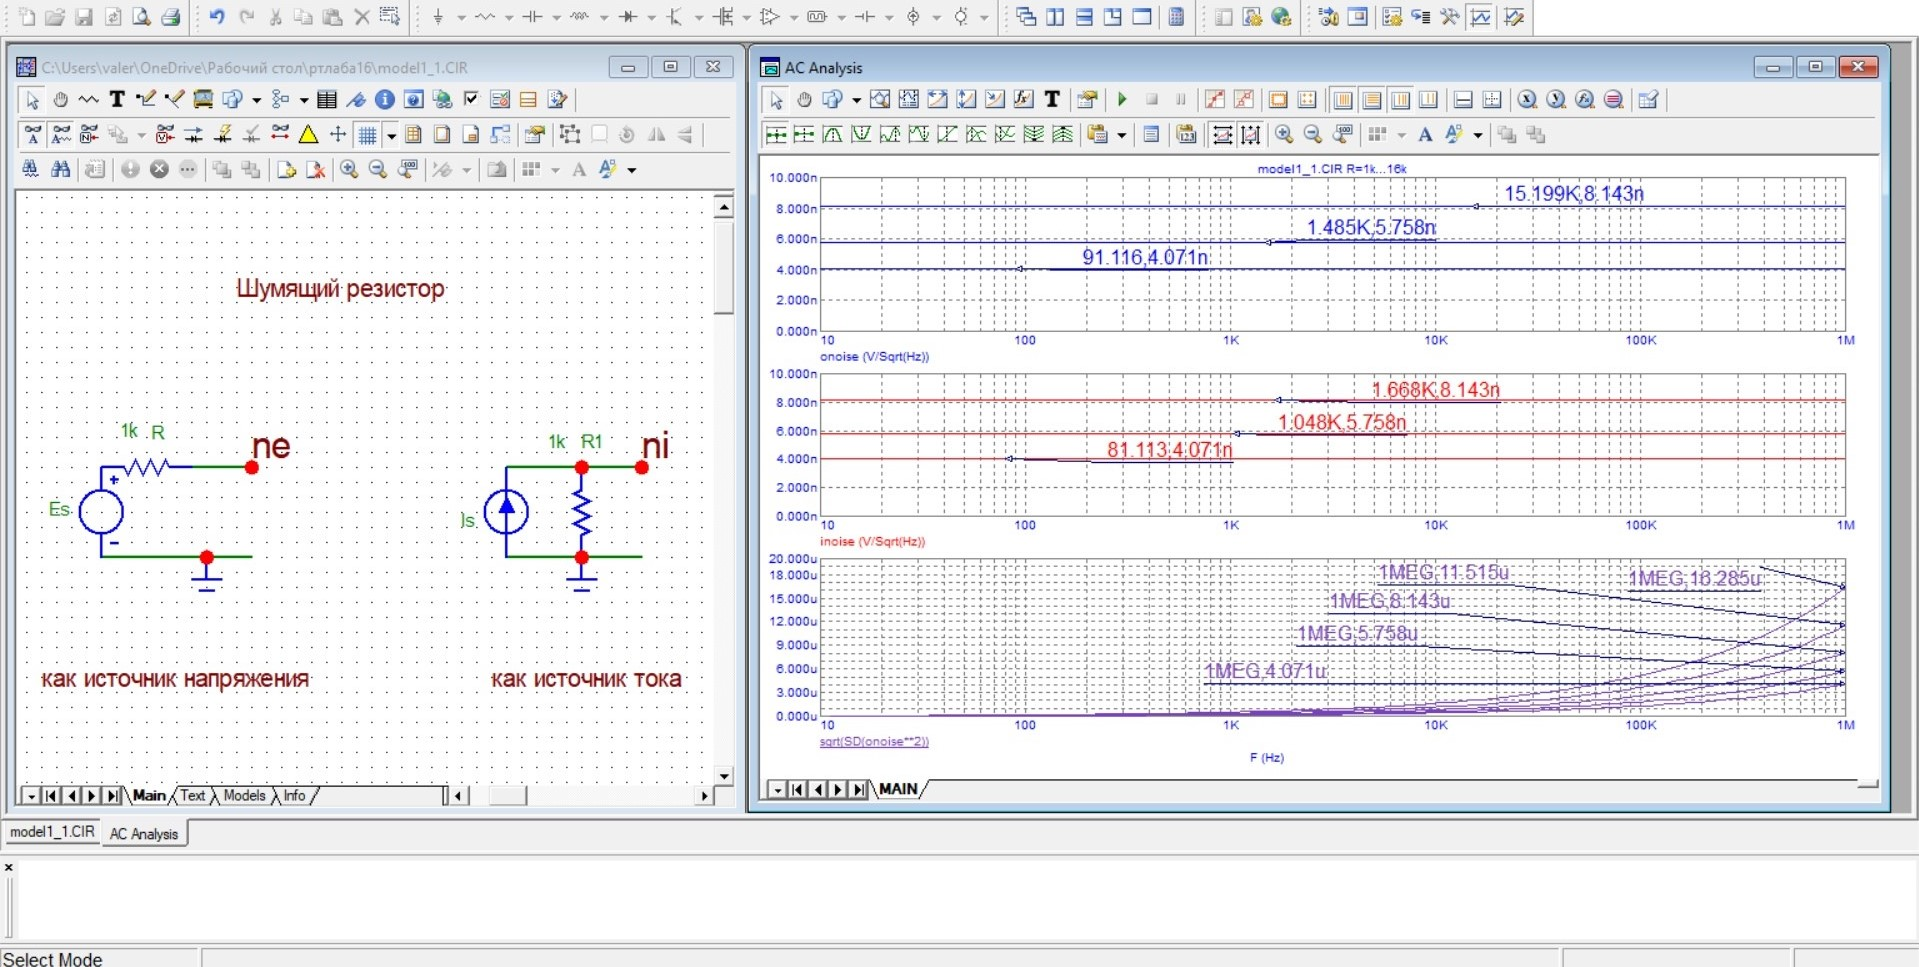
\includegraphics[width=0.3\textwidth]{./ann/3.PNG} 
\end{center}
\end{wrapfigure}

Равенство (2) может быть представлено графически (рис. 3) При разных $R$ графрики имеют вид прямых, пересекаЮщихся в точке $V=U, I=0 .$ Область, где эти иагрузочиъе прямвие пересекают вольт-амперную характеристику лампы, соответствует стационарному режиму - при малых $R$ (прямая 1$)$ лампа горит постоянно, колебания Отсутствуют. Прямая $2,$ проходящая через точку $\left(I_{2}, V_{2}\right),$ соответствует критическому сопротивлению
$$
R_{\mathrm{Kp}}=\frac{U-V_{2}}{I_{2}}
$$
При сопротивлении $R>R_{\text {кр }}$ нагрузочная прямая $3 \quad$ не пересекает характеристику лампы, поэтому стационарный режим невозможен. В этом случае в системе устанавливаются колебания. Рассмотрим, как происходит колебательный процесс. Пусть в начале опыта ключ К разомкнут (рис. 2) и $V=0 .$ Замкнём ключ. Конденсатор $C$ начинает заряжаться через сопротивление $R,$ напряжение на нём увеличивается (рис. 4) Как только оно достигнет напряжения зажигания $V_{1},$ лампа начинает проводить ток, причём прохождение тока сопровождается разрядкой конденсатора. В самом деле, батарея $U,$ подключённая через большое сопротивление $R,$ не может поддерживать необходимую для горения лампы величину тока. Во время горения лампы конденсатор разряжается, и когда напряжение на нём достигнет потенциала гашения, лампа перестанет проводить ток, а конденсатор вновь начнёт заряжаться. Возникают релаксационные колебания с амплитудой, равной $\left(V_{1}-V_{2}\right) .$

\newpage

\begin{wrapfigure}{r}{0.3\textwidth} 
\begin{center}
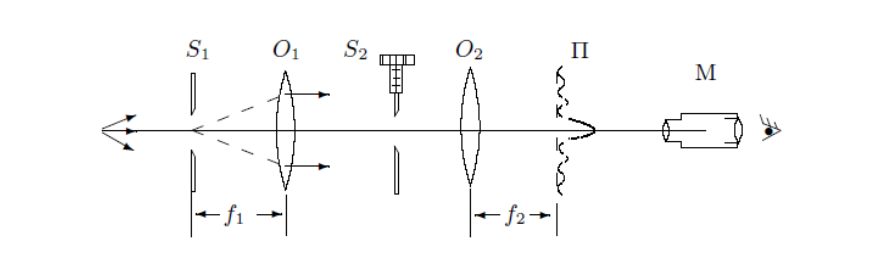
\includegraphics[width=0.3\textwidth]{./ann/4.PNG} 
\end{center}
\end{wrapfigure}

Рассчитаем период колебаний. Полное время одного периода колебаний Т состоит из суммы времени зарядки $\tau_{3}$ и времени разрядки $\tau_{\mathrm{p}},$ но если сопротивление $R$ существенно превосходит сопротивление Зажжённой лампы, то $\tau_{3} \gg \tau_{\mathrm{p}}$ и $T \simeq \tau_{3}($ этим случаем мы и ограничимся). Во время зарядки конденсатора лампа не горит $[I(V)=0],$ и уравнение (1) приобретает вид
$$
R C \frac{d V}{d t}=U-V
$$
Будем отсчитывать время с момента гашения лампы, так что $V=V_{2}$ при $t=0$ (рис. 4$) .$ Решив уравнение $(4),$ найдём
$$
V=U-\left(U-V_{2}\right) e^{-t /(R C)}
$$
$\mathrm{B}$ момент зажигания $t=\tau_{3}, V=V_{1},$ поэтому
$$
V_{1}=U-\left(U-V_{2}\right) e^{-\tau_{3} /(R C)}
$$
Из уравнений (5) и (6) нетрудно найти период колебаний:
$$
T \approx \tau_{3}=R C \ln \frac{U-V_{2}}{U-V_{1}}
$$
Развитая выше теория является приближённой. Ряд принятых при расчётах упрощающих предположений оговорен в тексте. Следует иметь в виду, что мы полностью пренебрегли паразитными емкостями и индуктивностями схемы. Не
рассматривались также процессы развития разряда и деионизация при гашении. Поэтому теория справедлива лишь в тех случаях, когда в схеме установлена достаточно большая ёмкость и когда период колебаний существенно больше времени развития разряда и времени деионизации (практически $\gg 10^{-5}$ с). Кроме того, потенциал гашения $V_{2},$ взятый из статической вольт-амперной характеристики, может отличаться от потенциала гашения лампы, работающей в динамическом режиме релаксационных колебаний.

\section{Ход работы}
\subsection{Характеристика стабилитрона}

Установка со стабилитроном имеет встроенное сопротивление $r = 5,4$ кОм.

С помощью приведённой ниже схемы можно получить ВАХ стабилитрона, в частности измерить напряжения зажигания и гашения (с учётом петли Гистерезиса).

\begin{figure}[h!]
    \centering
    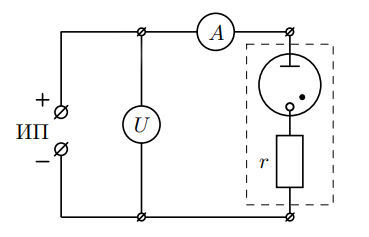
\includegraphics[width = 8 cm]{images/3.png}
    \caption{}
    \label{}
\end{figure}

Для этого снимем часть данных с приборов для построения ВАХ:

\begin{figure}[h!]
    \centering
    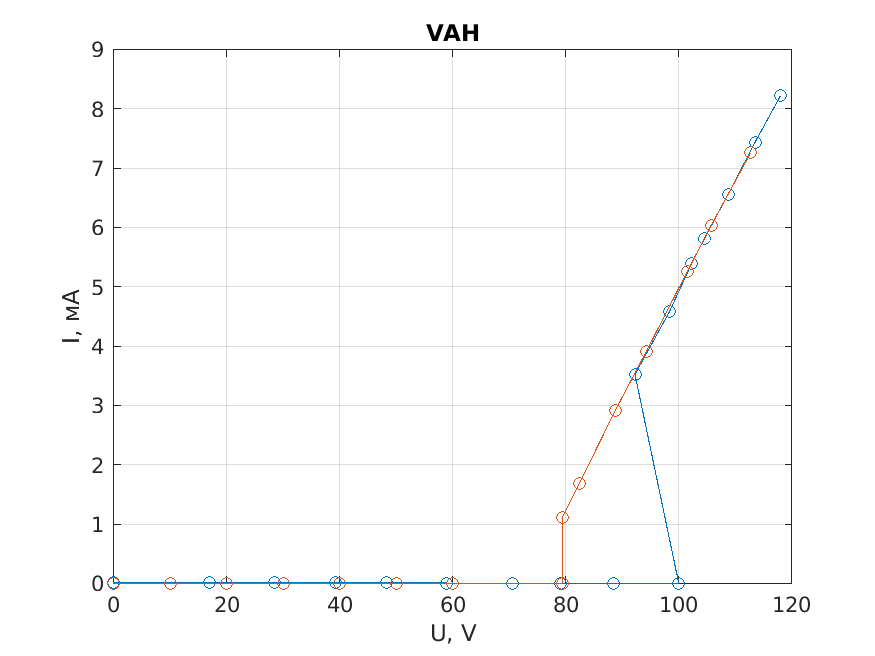
\includegraphics[width = 10 cm]{images/VAH.png}
    \caption{ВАХ стабилитрона}
    \label{vah}
\end{figure}

Здесь синяя кривая отвечает за увеличение напряжения, а оранжевая за уменьшение (рис. 4).

При этом график ВАХ стабилитрона без встроенного резистора имеет немного другой вид:

\begin{figure}[h!]
    \centering
    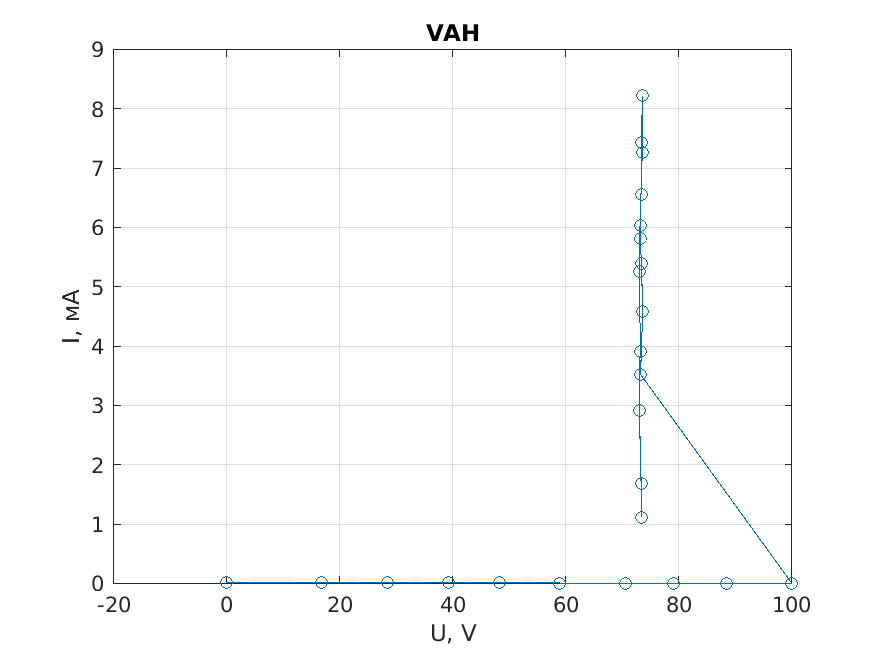
\includegraphics[width = 10 cm]{images/VAH2.png}
    \caption{ВАХ стабилитрона без учёта резистора}
    \label{vah2}
\end{figure}


Видно, что график вышел схожим по своей сути с теоретическим графиком.
Из него можно оценить напряжения зажигания и гашения, но для более точных значений проведём для этого несколько экспериментов и посчитаем среднее значение:

\begin{table}[h]
    \centering
    \begin{tabular}{|c|c|c|c|c|c|}
        \hline
        \textbf{$U_1, В$}  & 99,70 & 100,3  & 101,1  & 99,70 & 99,70 \\ \hline
        \textbf{$U_2, В$}  & 75,27 & 73,98  & 74,78  & 74,89 & 75,01 \\ \hline
        \textbf{$I_1, мА$} & 3,387 & 3,354  & 3,415  & 3,449 & 3,432 \\ \hline
        \textbf{$I_2, мА$} & 0,427 & 0,410  & 0,408  & 0,394 & 0,414 \\ \hline
    \end{tabular}
    \caption{Значения зажигания и гашения}
\end{table}

Итого имеем:

\begin{equation}
    U_1 = 100,1 \text{В}, \; \Delta  U_1 = 1,08 \text{В}
\end{equation}

\begin{equation}
    U_2 = 74,79 \text{В}, \; \Delta  U_2 = 0,95 \text{В}
\end{equation}

\begin{equation}
    I_1 = 3,407 \text{мA}, \; \Delta  I_1 = 0,058 \text{мA}
\end{equation}

\begin{equation}
    I_2 = 0,411 \text{мA}, \; \Delta  I_2 = 0,032 \text{мA}
\end{equation}

Погрешности были найдены через стандартное отклонение (среднеквадратичное значение) и являются погрешностями отдельного измерения. Также было учтено, что в статическом режиме измерения значение напряжения колебалось в пределах $0,46$ В, а значение силы тока в пределах $0,021$ мА.

\subsection{Времена гашения и зажигания}

Собрав схему, изоюражённую на рис. 1, установим сопротивление реостата $R = 900$ кОм, а ёмкость конденсатора $50$ нФ. Установив выходное напряжение источника питания $\varepsilon = 121 \pm 1$ В, установим по осциллограмме значения времён зарядки и разрядки:

\begin{equation}
    \tau_{\text{з}} = 39,5 \pm 0,5 \; \text{мс}
\end{equation}

\begin{equation}
    \tau_{\text{р}} = 0,65 \pm 0,05 \; \text{мс}
\end{equation}

Погрешности были учтены с помощью цены деления экрана осциллографа (в зависимости от масштаба развёртки -- $5$ $\text{ms/div}$ и $0,5$ $\text{ms/div}$ -- половина цены деления).

Для отношения времён имеем

\begin{equation}
    \frac{\tau_{\text{з}}}{\tau_{\text{р}}} = 60,7 \pm 1,2
\end{equation}

Очевидно, что суммарное время практически совпадает со значением времени зарядки $T = 40,15 \pm 0,55$ мс (погрешность посчитана по формуле косвенной погрешности через частные производные).

\subsection{Критический случай}

Определим критическое сопротивление реостата, при котором пропадают колебания в цепи: $R_{\text{крит}} = 138 \pm 1$ кОм.

При этом если сохранять значение сопротивления постоянным, а менять (уменьшать) значение исходного напряжения источника, то колебания тоже проадают при достижении некоторого значения.

\subsection{Исследование зависимости периода колебания цепи от её параметров}

Зафиксируем сопротивление реостата $R = 300$ кОм, вычислим, как зависит период колебания цепи от ёмкости конденсатора. В этом случае напряжение источника держим постоянным.
Зафиксировов экспериментальные значения и посчитав нужные теоретические значения, строим график.

\begin{figure}[h]
    \centering
    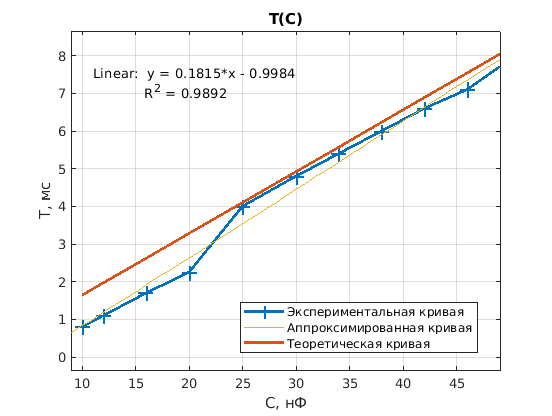
\includegraphics[width = 10 cm]{images/TC.png}
    \caption{Зависимость $T(C)$}
    \label{TC}
\end{figure}

\begin{figure}[h]
    \centering
    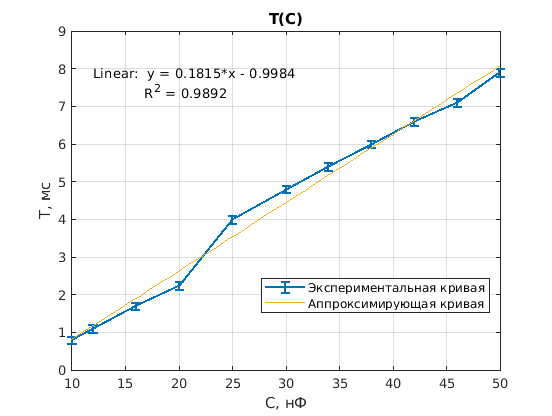
\includegraphics[width = 10 cm]{images/TC2.png}
    \caption{Зависимость $T(C)$ с ошибками измерения}
    \label{TC2}
\end{figure}

Видно, что вблизи центра рассмотренного набора значений графики почти совпадают, но на более низких ёмокстях происходит некоторый резкий спад периода. Возможно, он обсуловлен неточностью осциллографа. Значения ниже $10$ нФ не были рассмотрены, так как уже на этом этапе амплитуда колебаний на осциллографе заметно падает (вплоть до прекращения автоколебаний).

Для теоретической кривой коэффициент наклона равен $k = 0,158 \cdot 10^6$ с/Ф, для экспериментальной $(0,182 \pm 0,012) \cdot 10^6$ с/Ф. Значения различаются даже с учётом погрешности. В этом случае посчитаем динамический потенциал гашения $U_2$, воспользовавшись экспериментальной кривой и формулой:

\begin{equation}
    T = RC \ln{\frac{\varepsilon - U_2}{\varepsilon - U_1}} \Rightarrow U_2 = 82,3 \; \text{В}, \; \Delta U_2 = 2,1 \; \text{В}
\end{equation}

Погрешности для значения динамического потенциала гашения были найдены с помощью погрешности измерения $\varepsilon$, $k$ и стандартной формулы для погрешностей косвенных измерений.

Далее фиксируем ёмкость конденсатора $C = 50$ нФ, напряжение источника то же, что и было. Исследуем зависимость $T(R)$.

\begin{figure}[h!]
    \centering
    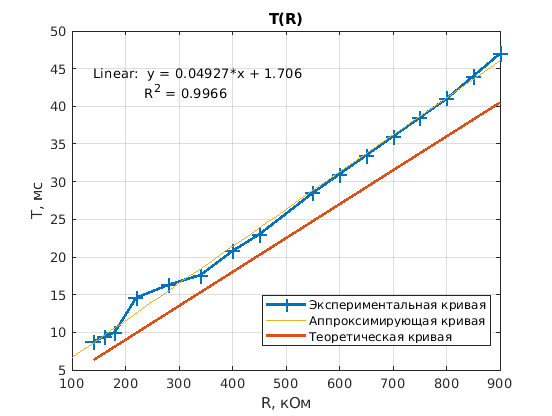
\includegraphics[width = 10 cm]{images/TR.png}
    \caption{Зависимость $T(R)$}
    \label{TR}
\end{figure}

\begin{figure}[h!]
    \centering
    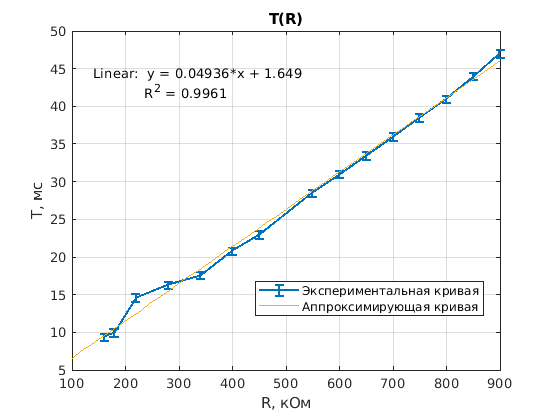
\includegraphics[width = 10 cm]{images/TR2.png}
    \caption{Зависимость $T(R)$ с ошибками измерения}
    \label{TR2}
\end{figure}

Видны флуктуации от прямой линии в районе $300$ кОм, которые не влияют на общий характер зависимости. Опять же, экспериментальная кривая почти совпадает с теоретической (характер зависимостей одинаков).

Для теоретической кривой коэффициент наклона равен $k = 44,5 \cdot 10^{-9}$ с/Ом, для экспериментальной $(49,3 \pm 2,1) \cdot 10^{-9}$ с/Ом. Значения аналогично различаются даже с учётом погрешности, как и для предыдущей зависимости. Посчитаем динамический потенциал гашения $U_2$:

\begin{equation}
    T = RC \ln{\frac{\varepsilon - U_2}{\varepsilon - U_1}} \Rightarrow U_2 = 84,8 \; \text{В}, \; \Delta U_2 = 1,7 \; \text{В}
\end{equation}


\section{Заключение}

Были найдены знчения напряжения и силы тока для зажигания и гашения для стабилитрона. 

Были найдены значения времён автоколебаний (в том числе отдельно для зажигания и гашения), в том числе зависимость времени автоколебания от ёмкости или сопротивления реостата в схеме.

Также частота могла быть найдена через фигуры Лиссажу, но в этом случае затруднительно найти отношения времён зажигания и гашения стабилитрона.


\section{Литература}

\begin{enumerate}
\item \textbf{Лабораторный практикум по общей физике:} учеб. пособие. В трёх томах. Т. 2. Электричество и магнетизм /
Никулин М. Г., Попов П. В., Нозик А. А., и др.; под ред. А. В. Мак­симычева, М. Г. Никулина. — 2-е изд., перераб. и доп. — Москва : МФТИ, 2019. — 370 с.
ISBN 978-5-7417-0709-8 (Т. 2. Электричество и магнетизм)
\end{enumerate}		
		

\end{document}
